\documentclass[a4paper, 12pt]{article}
\usepackage[utf8]{inputenc}
\usepackage[left=3cm, top=3cm, right=2cm, bottom=2cm]{geometry}%ajusta as margens
\usepackage{setspace}
\setlength{\parindent}{1.25cm}%Altera o parágrafo
\usepackage{graphicx}
\usepackage[portuguese]{babel} 
\usepackage{enumitem}
\setlist[itemize]{label=$\star$}
\begin{document}

\begin{center}
    \large
    \textbf{Faculdade de Tecnologia Baixada Santista Rubens Lara\\}
    \textbf{Curso Superior de Tecnologia em Ciência de Dados}
    \vspace{6.5cm}\\
    Anderson Portes do Nascimento\\Kaylane Chavier Costa\\
    \vspace{6cm}
    \textbf{PCA - Análise dos componentes principais}
    \\
    \vspace{6cm}
    Santos, SP\\
    2023
\end{center}

\newpage
    \onehalfspacing
    \section{Introdução}
    
    \par O tema escolhido para desenvolvimento do trabalho foi vinhos. Através de uma pesquisa bibliográfica, foi encontrado um dataset, no site Kaggle, dos tipos de vinho e suas respectivas qualidades e, através dele, foi realizado o PCA (análise dos componentes principais).



\section{Codificação}

\subsection{Passo 1 - Baixar o dataset via kaggle}

\\Acessando o link https://www.kaggle.com/datasets/yasserh/wine-quality-dataset é possível visualizar as informações sobre a base de dados utilizada e baixar o arquivo csv clicando em "Download".


\subsection{Passo 2 - Criar o arquivo .py ou .ipynb (notebook python)}

\\Cria-se os arquivos com extensão .py e .ipynb para realizar a codificação do PCA.

\subsection{Passo 3 - Importar as bibliotecas que serão utilizadas no desenvolvimento}

\\Importou-se as bibliotecas que serão utilizadas no desenvolvimento no arquivo .ipynb:

\begin{itemize}
  \begin{description}
    \item[import numpy as np:] Biblioteca do numpy usada para realizar as operações matematicas dentro do código;
    \item[import pandas as pd:] Biblioteca usada para importar a base de dados .csv;
    \item[import matplotlib.pyplot as plt:] Biblioteca usada para plotar os gráficos;
    \item[from sklearn.preprocessing import StandardScaler:] Biblioteca usada para normalizar os dados.
  \end{description}
\end{itemize}

 \begin{figure}[!ht]
        \centering
        \caption{Código do 3º passo}
        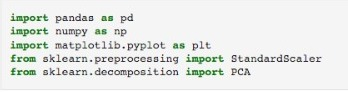
\includegraphics[scale=0.5]{passo3.jpg} \\
        {\footnotesize Fonte: Elaborada pelo autor.}
        \label{fig:my_label}
    \end{figure}

\newpage

\subsection{Passo 4 - Importar o dataset e remover dados nulos}

\\A função "pd.read csv" serve para importar o dataset dentro do código, neste caso, nomeado como "data.csv".
A função "dropna" remove os dados nulos do dataset o parametro "inplce=true" indica que a própria variavel
"data" será reescrita.

     \begin{figure}[!ht]
        \centering
        \caption{Código do 4º passo}
        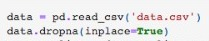
\includegraphics[scale=0.5]{passo4.jpg} \\
        {\footnotesize Fonte: Elaborada pelo autor.}
        \label{fig:my_label}
    \end{figure}

\newpage
\subsection{Passo 5 - Criação de labels para, posteriormente, distinguir a qualidade dos vinhos}

\\A variavel "mean quality" contém a media de qualidade dos vinhos, enquanto a variavel "is good"
será um vetor contendo apenas "True" ou "False", indicando se a qualidade do vinho do índice está
maior ou igual a média de qualidade, exemplificando caso o indice 0 dessa variável for "True", logo
o primeiro vinho possuí uma qualidade maior ou igual a média.

 \begin{figure}[!ht]
        \centering
        \caption{Código do 5º passo}
        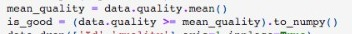
\includegraphics[scale=0.5]{passo5.jpg} \\
        {\footnotesize Fonte: Elaborada pelo autor.}
        \label{fig:my_label}
    \end{figure}

\subsection{Passo 6 - Remover colunas desnecessárias}

\\De início, o dataset contém duas colunas que não serão utilizadas na análise: a "quality" - esse será o ponto de análise, por isso ela será retirada do dataset -
e a "Id", que não contribui na análise.
\\a função drop recebe como primeiro parametro um array com o nome das colunas que serão removidas. O "axis=1" indica que todos os elementos dessa coluna serão removidos e o "inplace=True" indica
que a variavel será reescrita.
 \begin{figure}[!ht]
        \centering
        \caption{Código do 6º passo}
        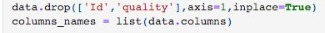
\includegraphics[scale=0.5]{passo6.jpg} \\
        {\footnotesize Fonte: Elaborada pelo autor.}
        \label{fig:my_label}
    \end{figure}

\subsection{Passo 7 - Transformar o dataset do pandas em uma estrutura do numpy e realizar a normalização dos dados}

\\A função "data.to numpy" transforma o dataframe do pandas em uma matriz do numpy, e, logo abaixo,
usa-se a classe "StandarScaler", executando a função "fit transform" para normalizar os elementos da
matriz onde a formula sera:

\\(valor do elemento - média) / desvio padrão

\\Com isso, os dados estarão na mesma escala.

 \begin{figure}[!ht]
        \centering
        \caption{Código do 7º passo}
        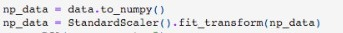
\includegraphics[scale=0.5]{passo7.jpg} \\
        {\footnotesize Fonte: Elaborada pelo autor.}
        \label{fig:my_label}
    \end{figure}

\subsection{Passo 8 - Realizar a decomposição por valores singulares}

\\a função "np.linalg.svd" retorna uma tripla, contendo as matrizes "U", "S" e "Vt". Neste caso, só
precisará da matriz "Vt" dos componentes pricipais.

 \begin{figure}[!ht]
        \centering
        \caption{Código do 8º passo}
        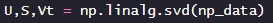
\includegraphics[scale=0.5]{passo8.png} \\
        {\footnotesize Fonte: Elaborada pelo autor.}
        \label{fig:my_label}
    \end{figure}

\begin{itemize}
  \begin{description}
    \item[import streamlit as st:] Para criar a interface;
    \item[import pickle:] Para ler as variaveis em memória;
    \item[import pandas as pd:] Para importar a base de dados.
  \end{description}
\end{itemize}

\subsection{Passo 9 - Projetar os 5 principais componentes na matriz inicial}

\\A variável "principal components" será uma matriz contendo os 5 principais componentes. Já a variavel "pca data" será a projeção entre a matriz inicial e os componentes principais.

 \begin{figure}[!ht]
        \centering
        \caption{Código do 9º passo}
        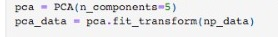
\includegraphics[scale=0.5]{passo9.jpg} \\
        {\footnotesize Fonte: Elaborada pelo autor.}
        \label{fig:my_label}
    \end{figure}
    
\newpage

\subsection{Passo 10 - Plotar todas as combinações dos principais componentes usando o scatterplot 2d}
\\Esse código realizará a comparação entre cada componente principal a partir de um gráfico "scatterplot" e, passando a variável "color"s dentro do plot, será possivel observar os vinhos com qualidade abaixo da média (pontos em vermelho) e os vinhos com qualidade acima ou igual a média (pontos azuis).

 \begin{figure}[!ht]
        \centering
        \caption{Código do 10º passo}
        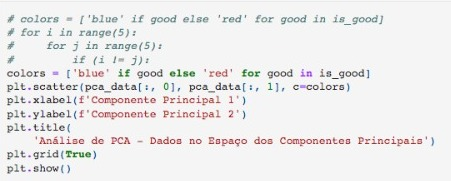
\includegraphics[scale=0.5]{passo10.jpg} \\
        {\footnotesize Fonte: Elaborada pelo autor.}
        \label{fig:my_label}
    \end{figure}
    
\newpage

\section{Resultado}
O melhor padrão encontrado foi utilizando, respectivamente, os principais componentes: 2, 4 e 3, onde pode-se observar o agrupamento de vinhos com qualidade abaixo da média - vermelhos - e os vinhos com qualidade igual ou acima da  média - azuis.
\begin{figure}[!ht]
        \centering
        \caption{Resultado}
        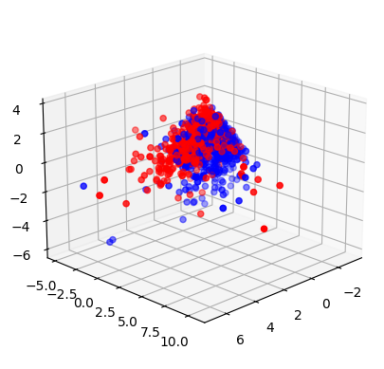
\includegraphics[scale=0.5]{grafico.png} \\
        {\footnotesize Fonte: Elaborada pelo autor.}
        \label{fig:my_label}
    \end{figure}


\newpage

\section{REPOSITÓRIO DO PROJETO}
Anderson Portes do Nascimento:
    \url{https://github.com/Anderson-Portes/wine-quality-pca}
\\\\Kaylane Chavier Costa:
    \url{https://github.com/kaychavier/wine-quality-pca}
\\\\Dataset:
\url{https://www.kaggle.com/datasets/yasserh/wine-quality-dataset}
\end{document}
%